\subsection{Validating MLMC Stochastic Heat Implementation}\label{sec:stoch_heat_validation}

This section presents the numerical validation of our MLMC implementation for the Stochastic Heat Equation. 
We do this by demonstrating that the MLMC estimator converges to the correct, 
analytically-derived expected value for quantities of interest, and that the observed 
error and variance decay rates align with theory.

We focus first on the squared amplitude of the first Fourier mode. The true value we know to 
be $0.10$
via \eqref{eq:squared_amplitude_analytic}.
For each of the three coupling strategies (NN, CC, and FE) the following was done. 
A preliminary run with 20,000 samples across six levels was performed to obtain 
empirical estimates of the key MLMC 
parameters ($\alpha, \beta, \gamma$) via linear regression. 
The adaptive MLMC algorithm (Algoritm \ref{alg:mlmc_detailed}) was then executed for a range of 
target RMSEs, $\varepsilon \in \{0.1, 0.05, 0.02, 0.01, 0.005, 0.001\}$. This is in line with the 
method outlined in Section
\ref{sec:mlmc_algorithm}.

The results of this analysis are presented in Figure \ref{fig:she_validation_combined}, 
with the estimated decay rates summarised in Table \ref{tab:she_decay_rates}.

\begin{figure}[htbp]
    \centering
    \begin{subfigure}{\textwidth}
        \centering
        \begin{subfigure}[b]{0.48\textwidth}
            \centering
            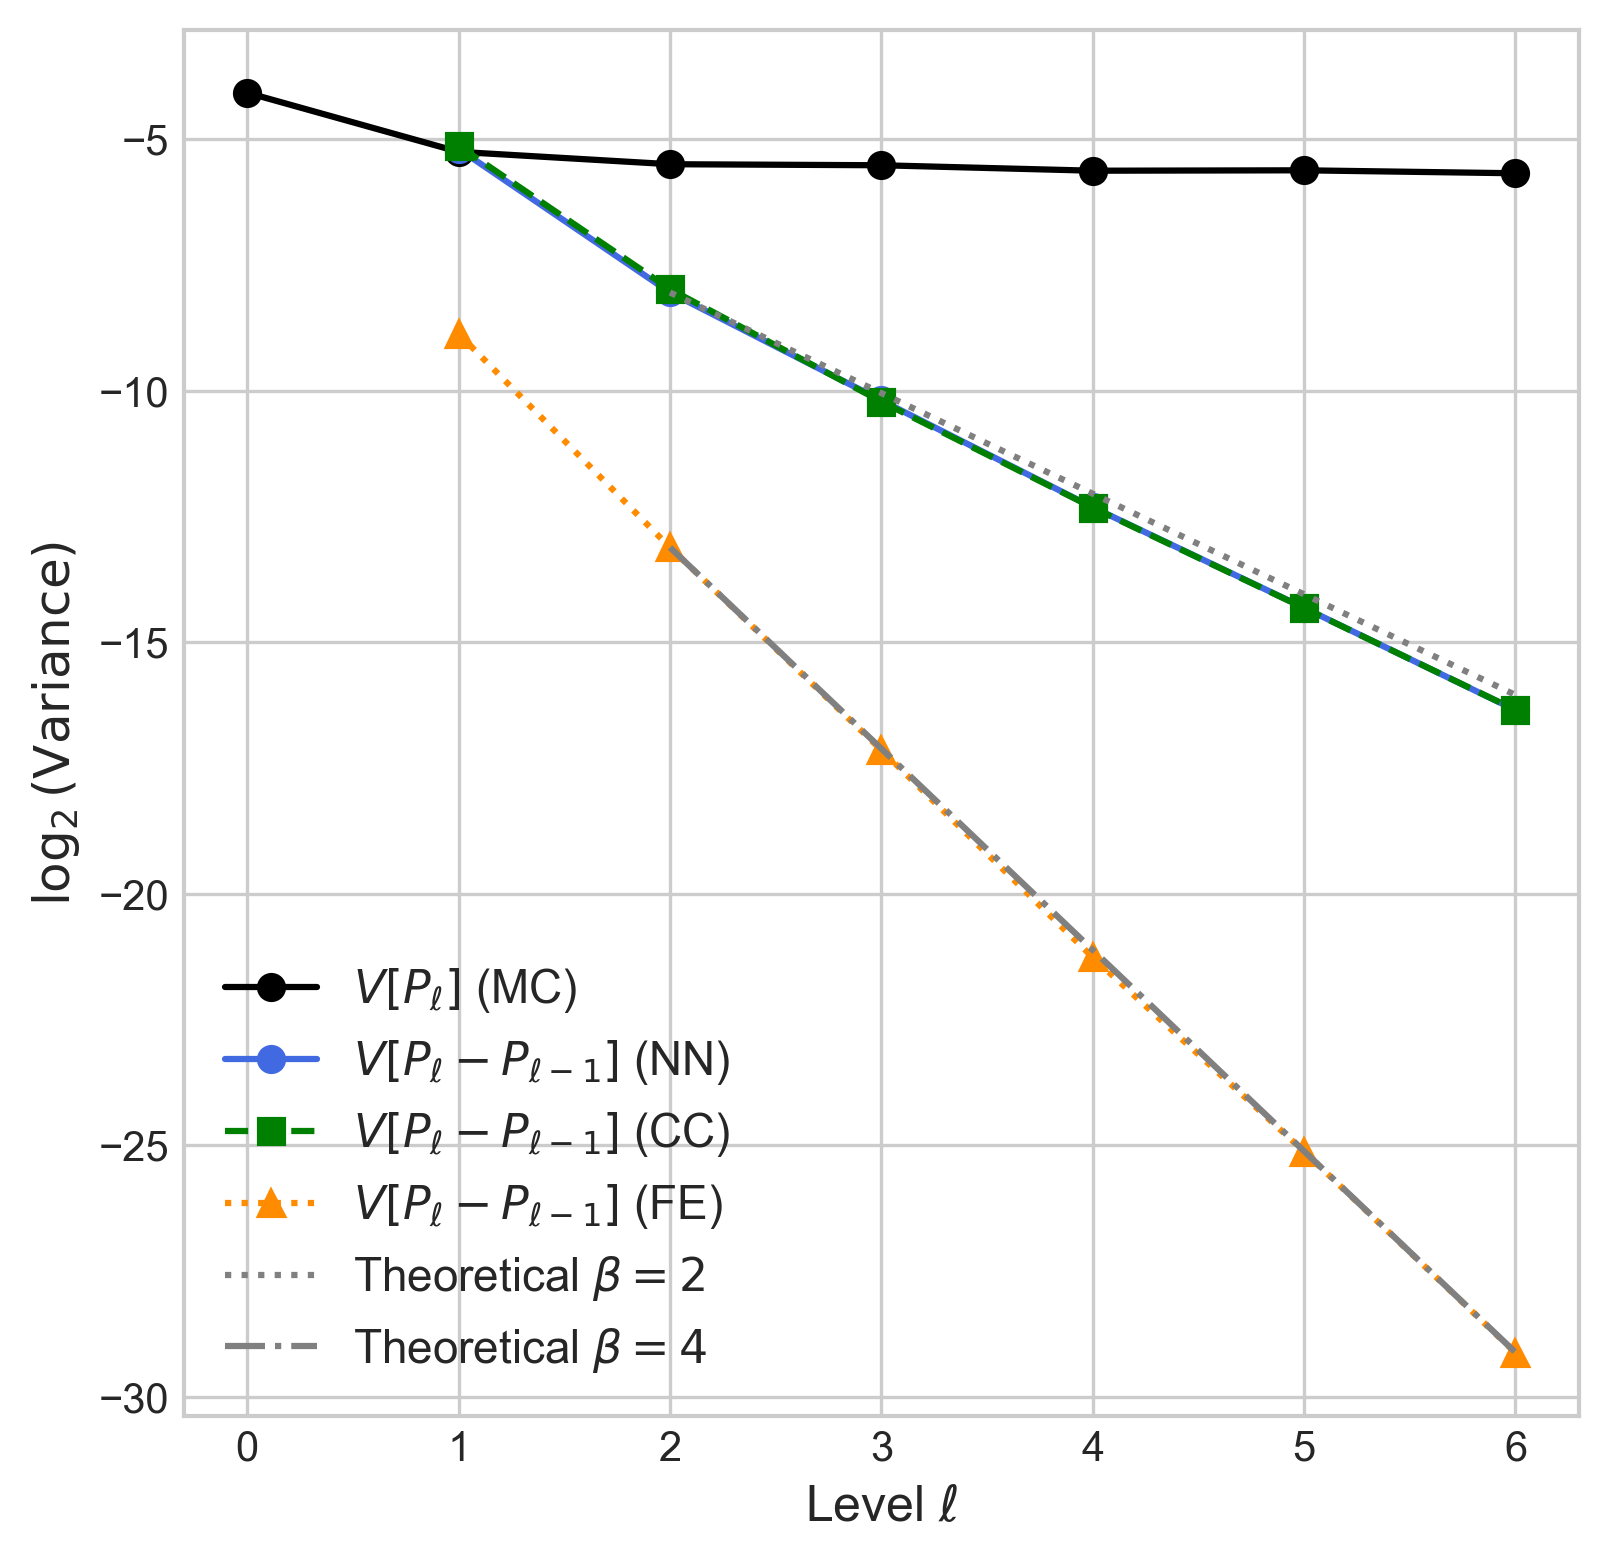
\includegraphics[width=\linewidth]{graphics/she_sq_amp_var_decay.png}
            \caption{MLMC variance decay ($\beta$).}
            \label{fig:variance_decay}
        \end{subfigure}
        \hfill
        \begin{subfigure}[b]{0.48\textwidth}
            \centering
            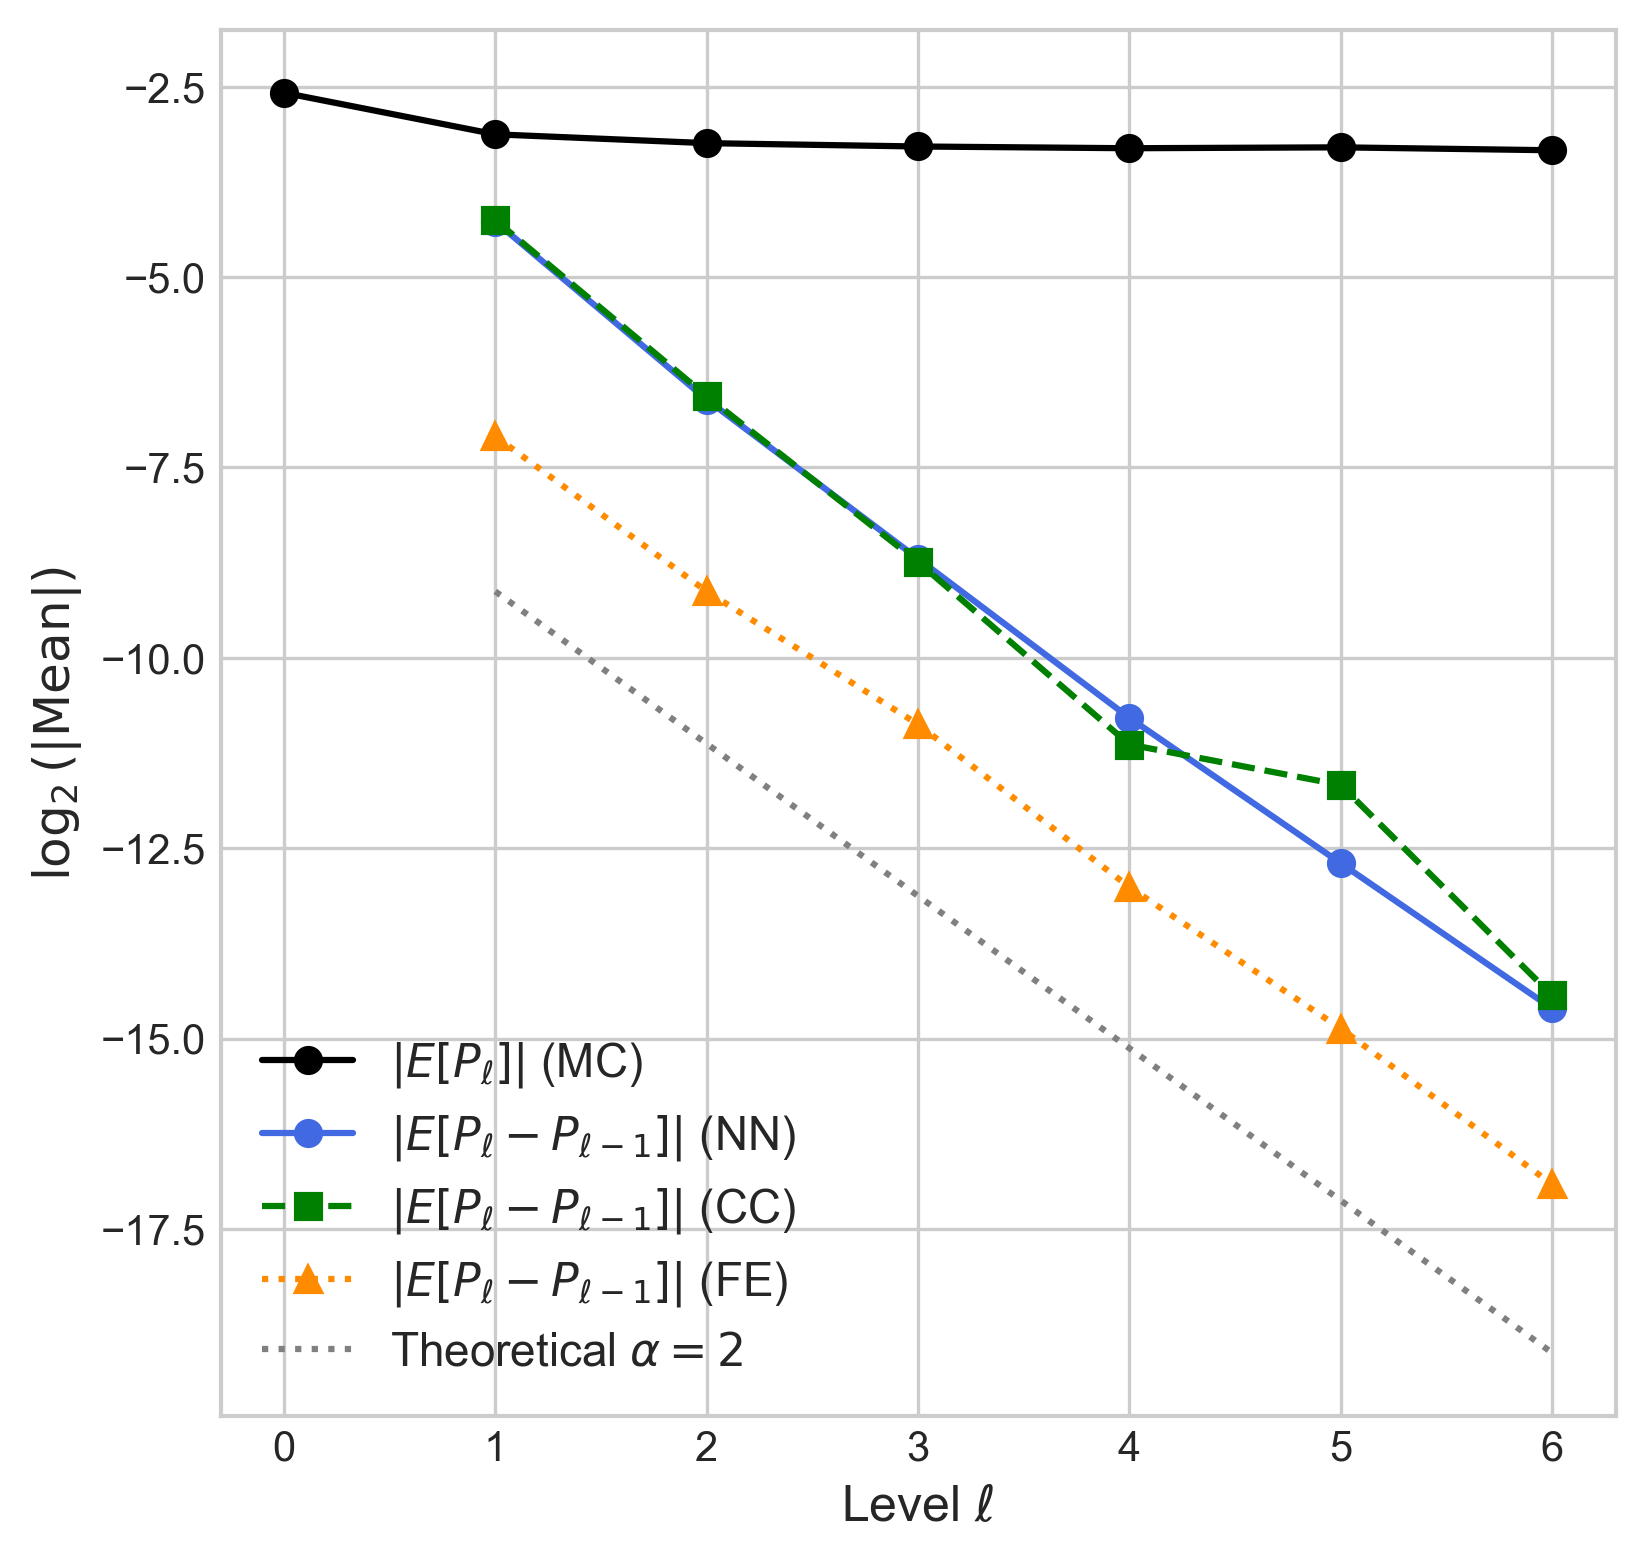
\includegraphics[width=\linewidth]{graphics/she_sq_amp_err_decay.png}
            \caption{Weak error convergence ($\alpha$).}
            \label{fig:mean_decay}
        \end{subfigure}
    \end{subfigure}
    \vspace{1cm}
    \begin{subfigure}{\textwidth}
        \centering
        \begin{subfigure}[b]{\textwidth}
            \centering
            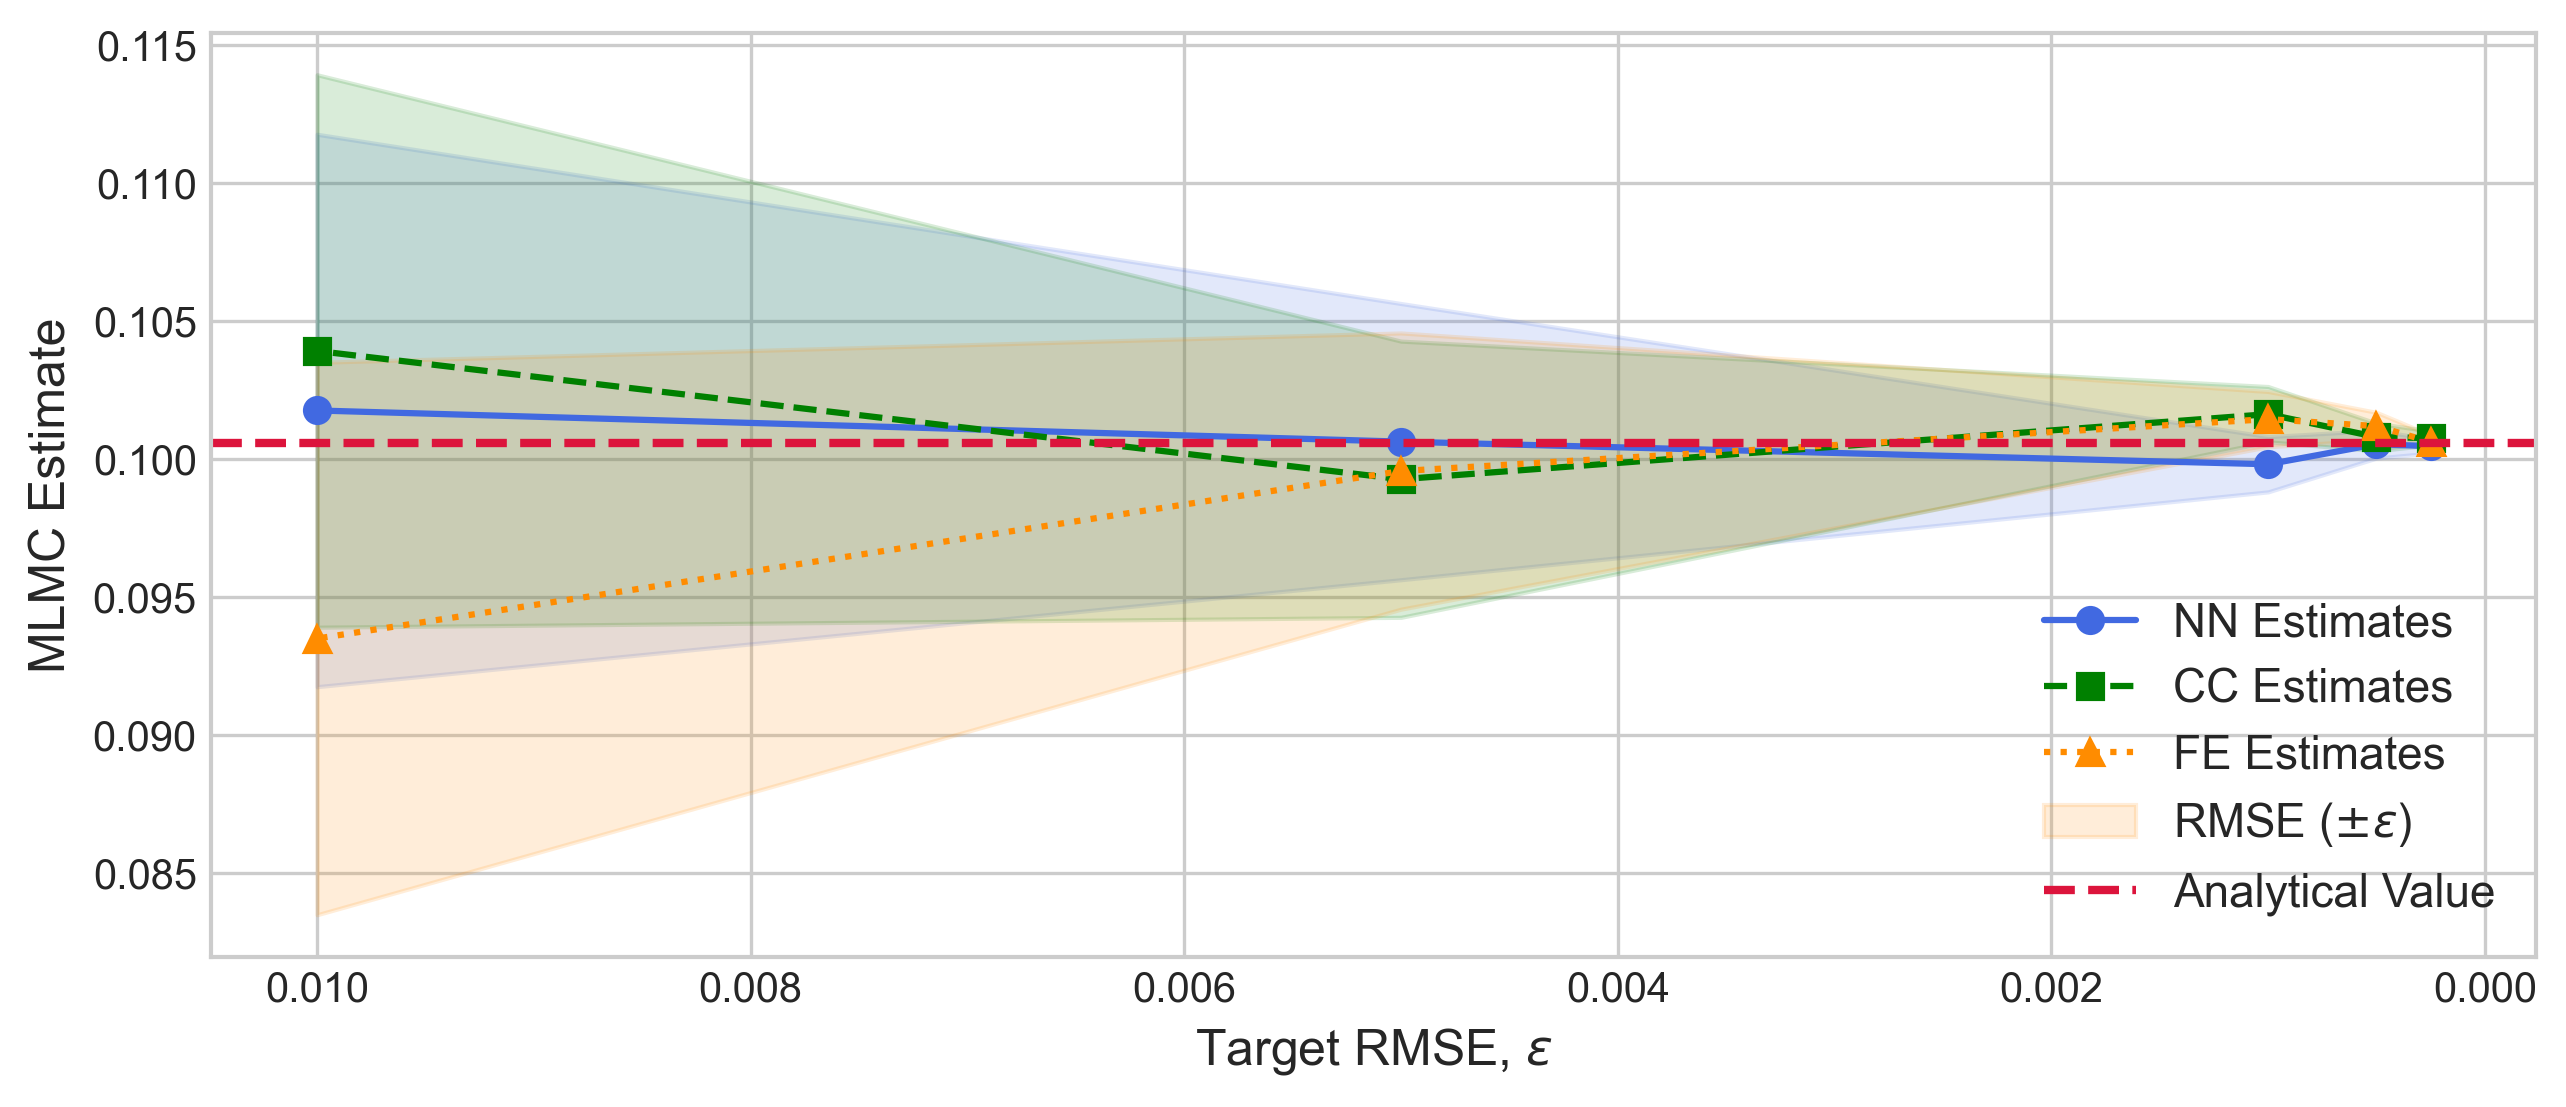
\includegraphics[width=0.7\linewidth]{graphics/she_sq_amp_conv.png}
            \caption{Final MLMC estimate vs. target RMSE ($\varepsilon$).}
            \label{fig:conv_vs_eps}
        \end{subfigure}
        \vspace{0.5cm}
        \begin{subfigure}[b]{\textwidth}
            \centering
            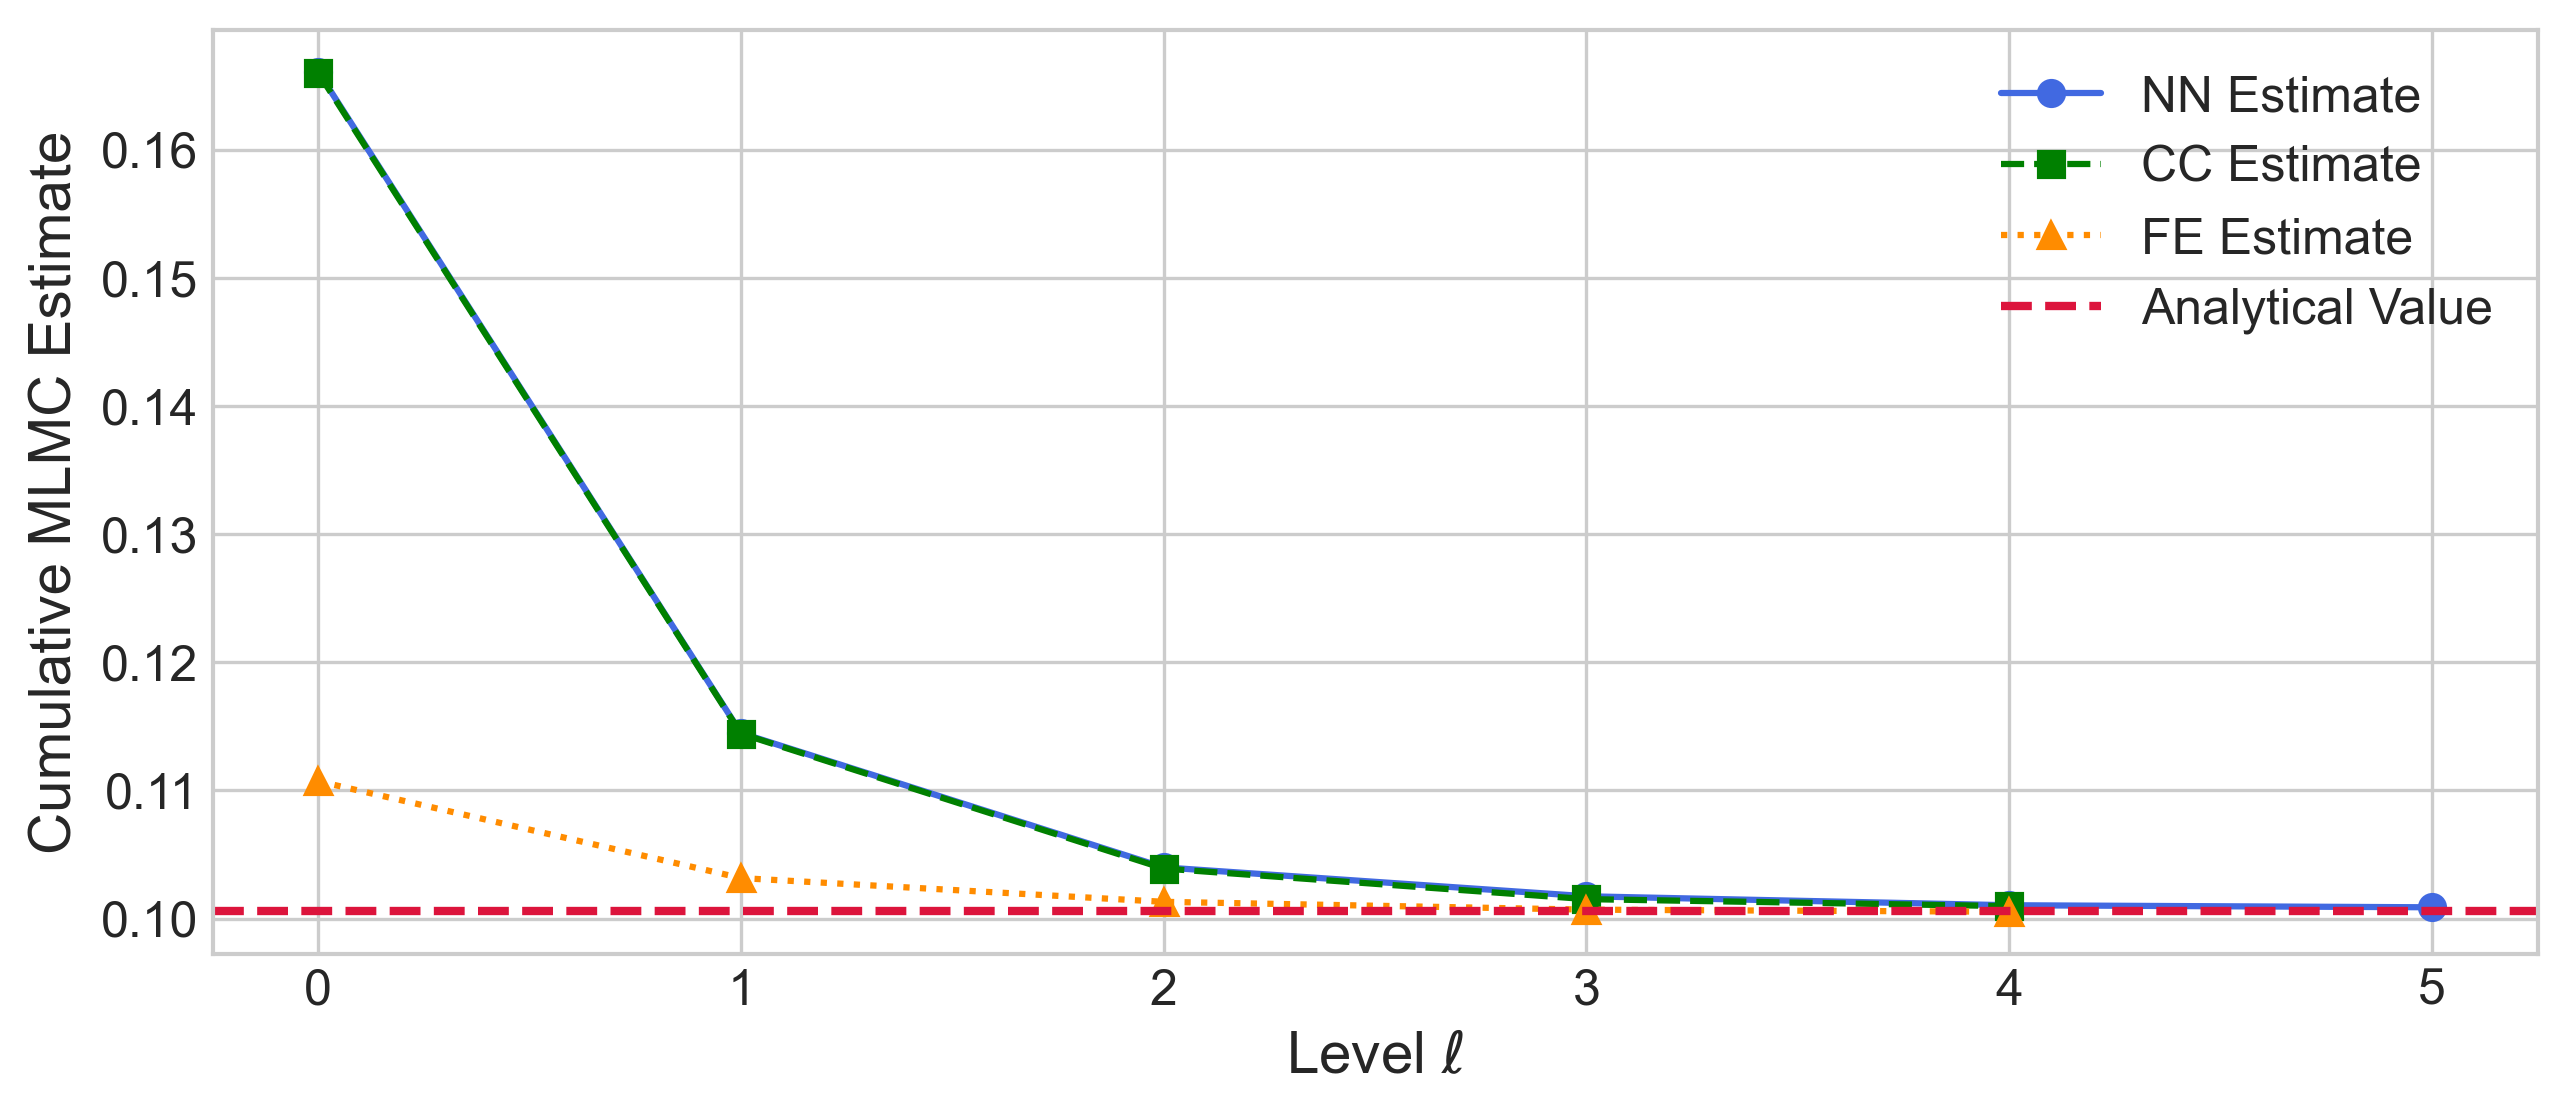
\includegraphics[width=0.7\linewidth]{graphics/she_sq_amp_cumconv.png}
            \caption{Cumulative estimate vs. level ($\ell$) for $\varepsilon=0.001$.}
            \label{fig:cumulative_conv}
        \end{subfigure}
    \end{subfigure}
    \caption{Validation and convergence plots for the MLMC implementation for the SHE, using the squared 
    amplitude of the first Fourier mode as our QoI.}
    \label{fig:she_validation_combined}
\end{figure}

\begin{table}[htbp]
    \centering
    \begin{tabular}{|l|c|c|r|}
        \hline
        \textbf{Coupling Method} & \textbf{$\alpha$} & \textbf{$\beta$} & \textbf{$\gamma$} \\
        \hline
        Nearest Neighbour & 2.0 & 2.07 & 3.02\\
        Central Coupling & 1.86 & 2.08 & 3.02 \\
        Finite Element & 1.96 & 4.0 & 3.0 \\
        \hline
    \end{tabular}
    \caption{Empirically estimated rates for the Squared Amplitude QoI.}
    \label{tab:she_decay_rates}
\end{table}


Figures \ref{fig:conv_vs_eps} and \ref{fig:cumulative_conv} 
show that the MLMC estimates for all three coupling strategies converge to the true 
value. 


The decay rate plots align with our theoretical predictions from Propositions 
\ref{prop:weak_error_for_fourier_mode} and \ref{prop:variance_decay_fourier}. 
The weak error for all methods, shown in Figure \ref{fig:mean_decay},
converges with a rate of $\alpha \approx 2$, consistent with 
the expected $\mathcal{O}((\Delta x)^2)$ convergence.

The variance decay plot in Figure \ref{fig:variance_decay} highlights the critical 
difference between the coupling strategies. The NN and CC methods 
both exhibit a variance decay of $\beta \approx 2$, which aligns with the theoretical rate 
for imperfectly correlated processes. In contrast, the FE coupling 
method achieves a much faster decay rate of $\beta \approx 4$. This confirms that the 
mathematically-grounded coupling derived from the FEM basis functions achieves the optimal
rate for this quantity of interest.




\begin{figure}[htbp]
    \centering
    \begin{subfigure}{\textwidth}
        \centering
        \begin{subfigure}[b]{0.48\textwidth}
            \centering
            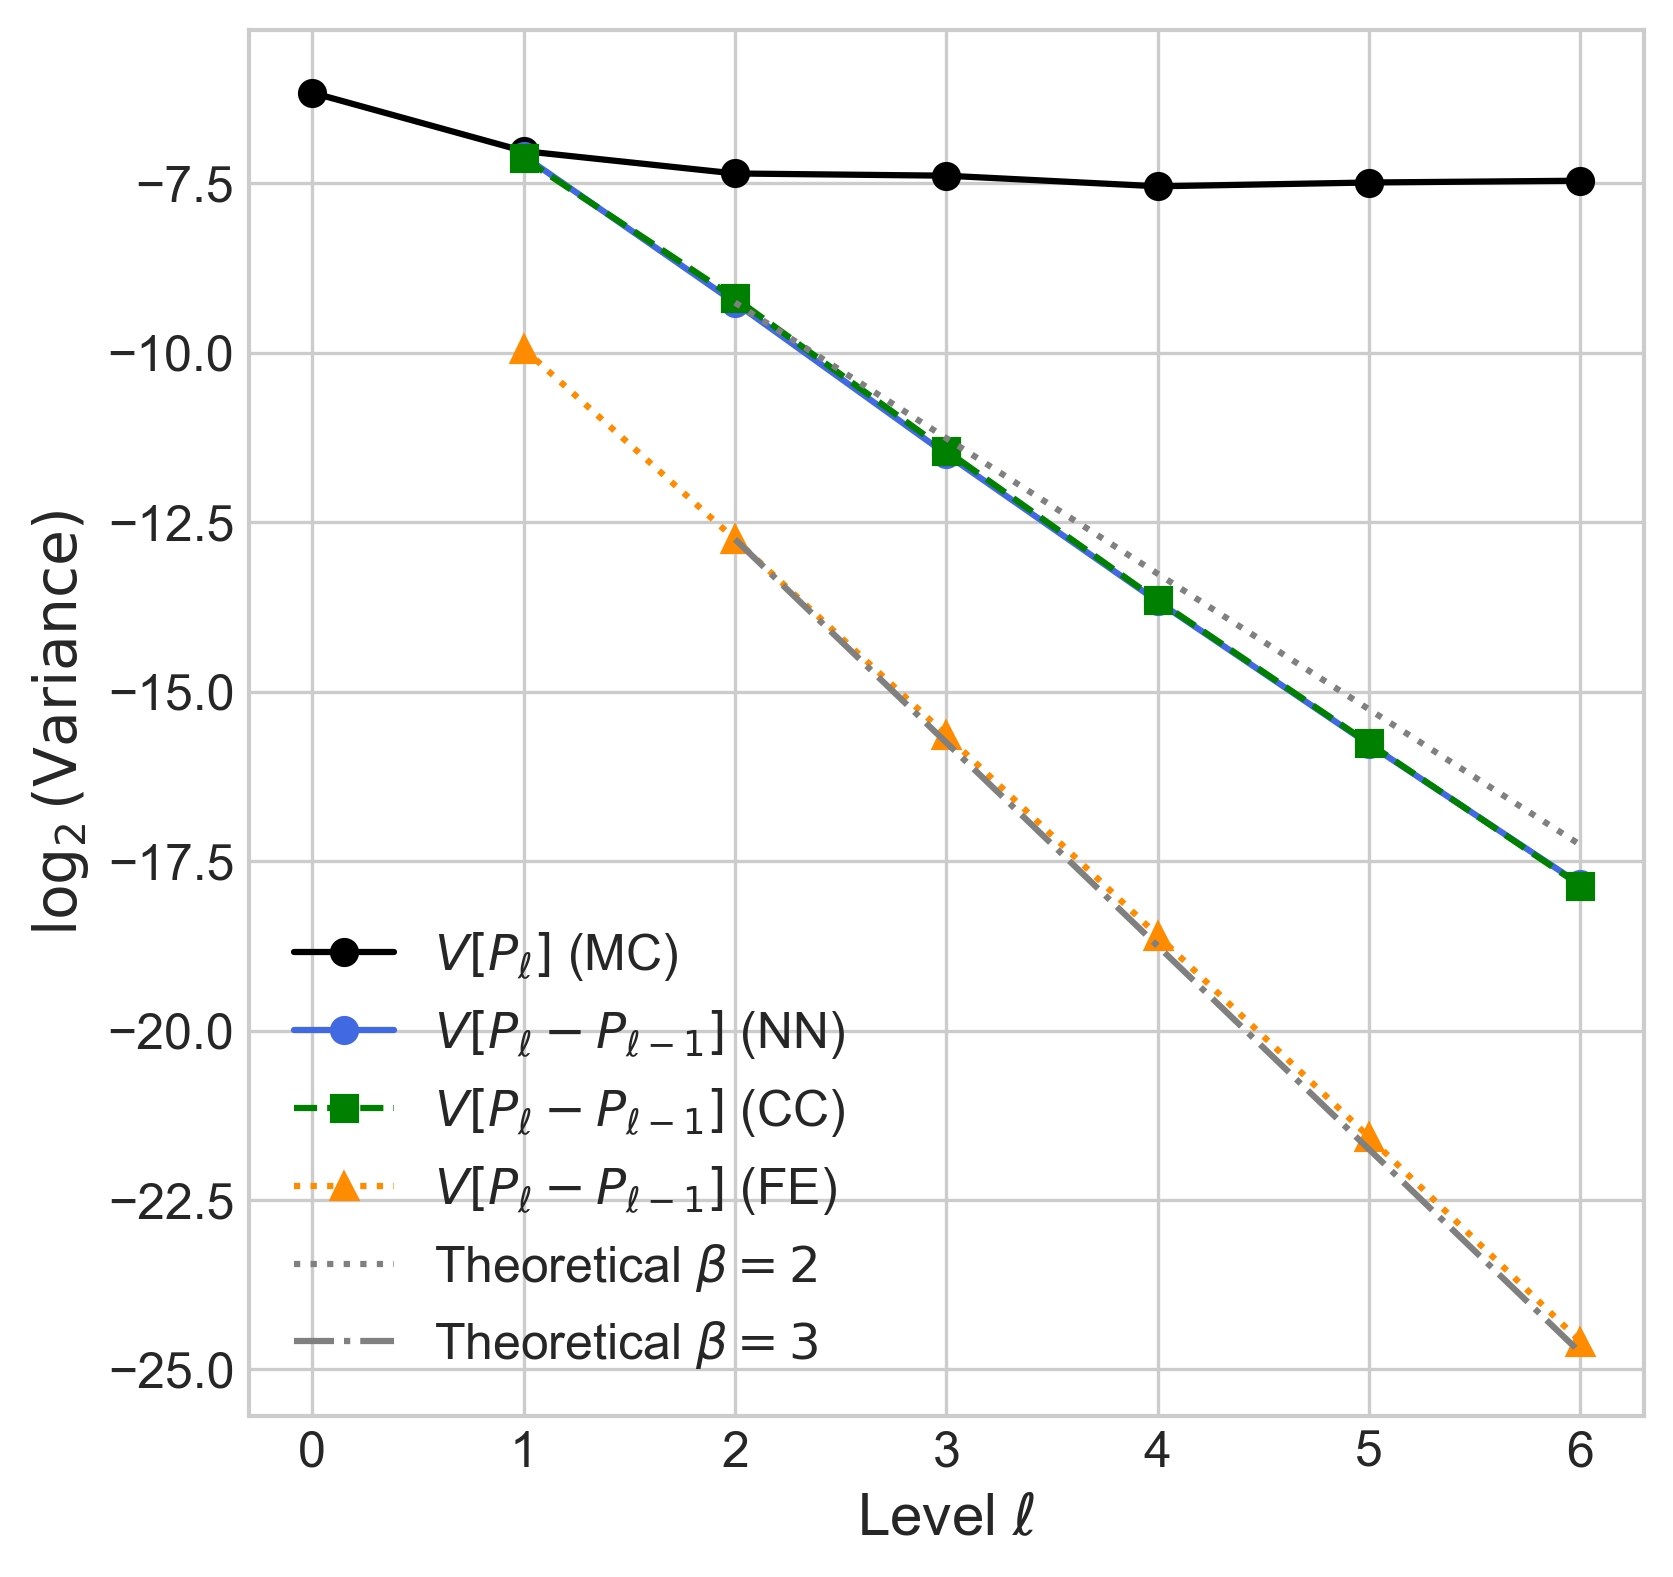
\includegraphics[width=\linewidth]{graphics/she_energy_var_decay.png}
            \caption{MLMC variance decay ($\beta$).}
            \label{fig:variance_decay}
        \end{subfigure}
        \hfill
        \begin{subfigure}[b]{0.48\textwidth}
            \centering
            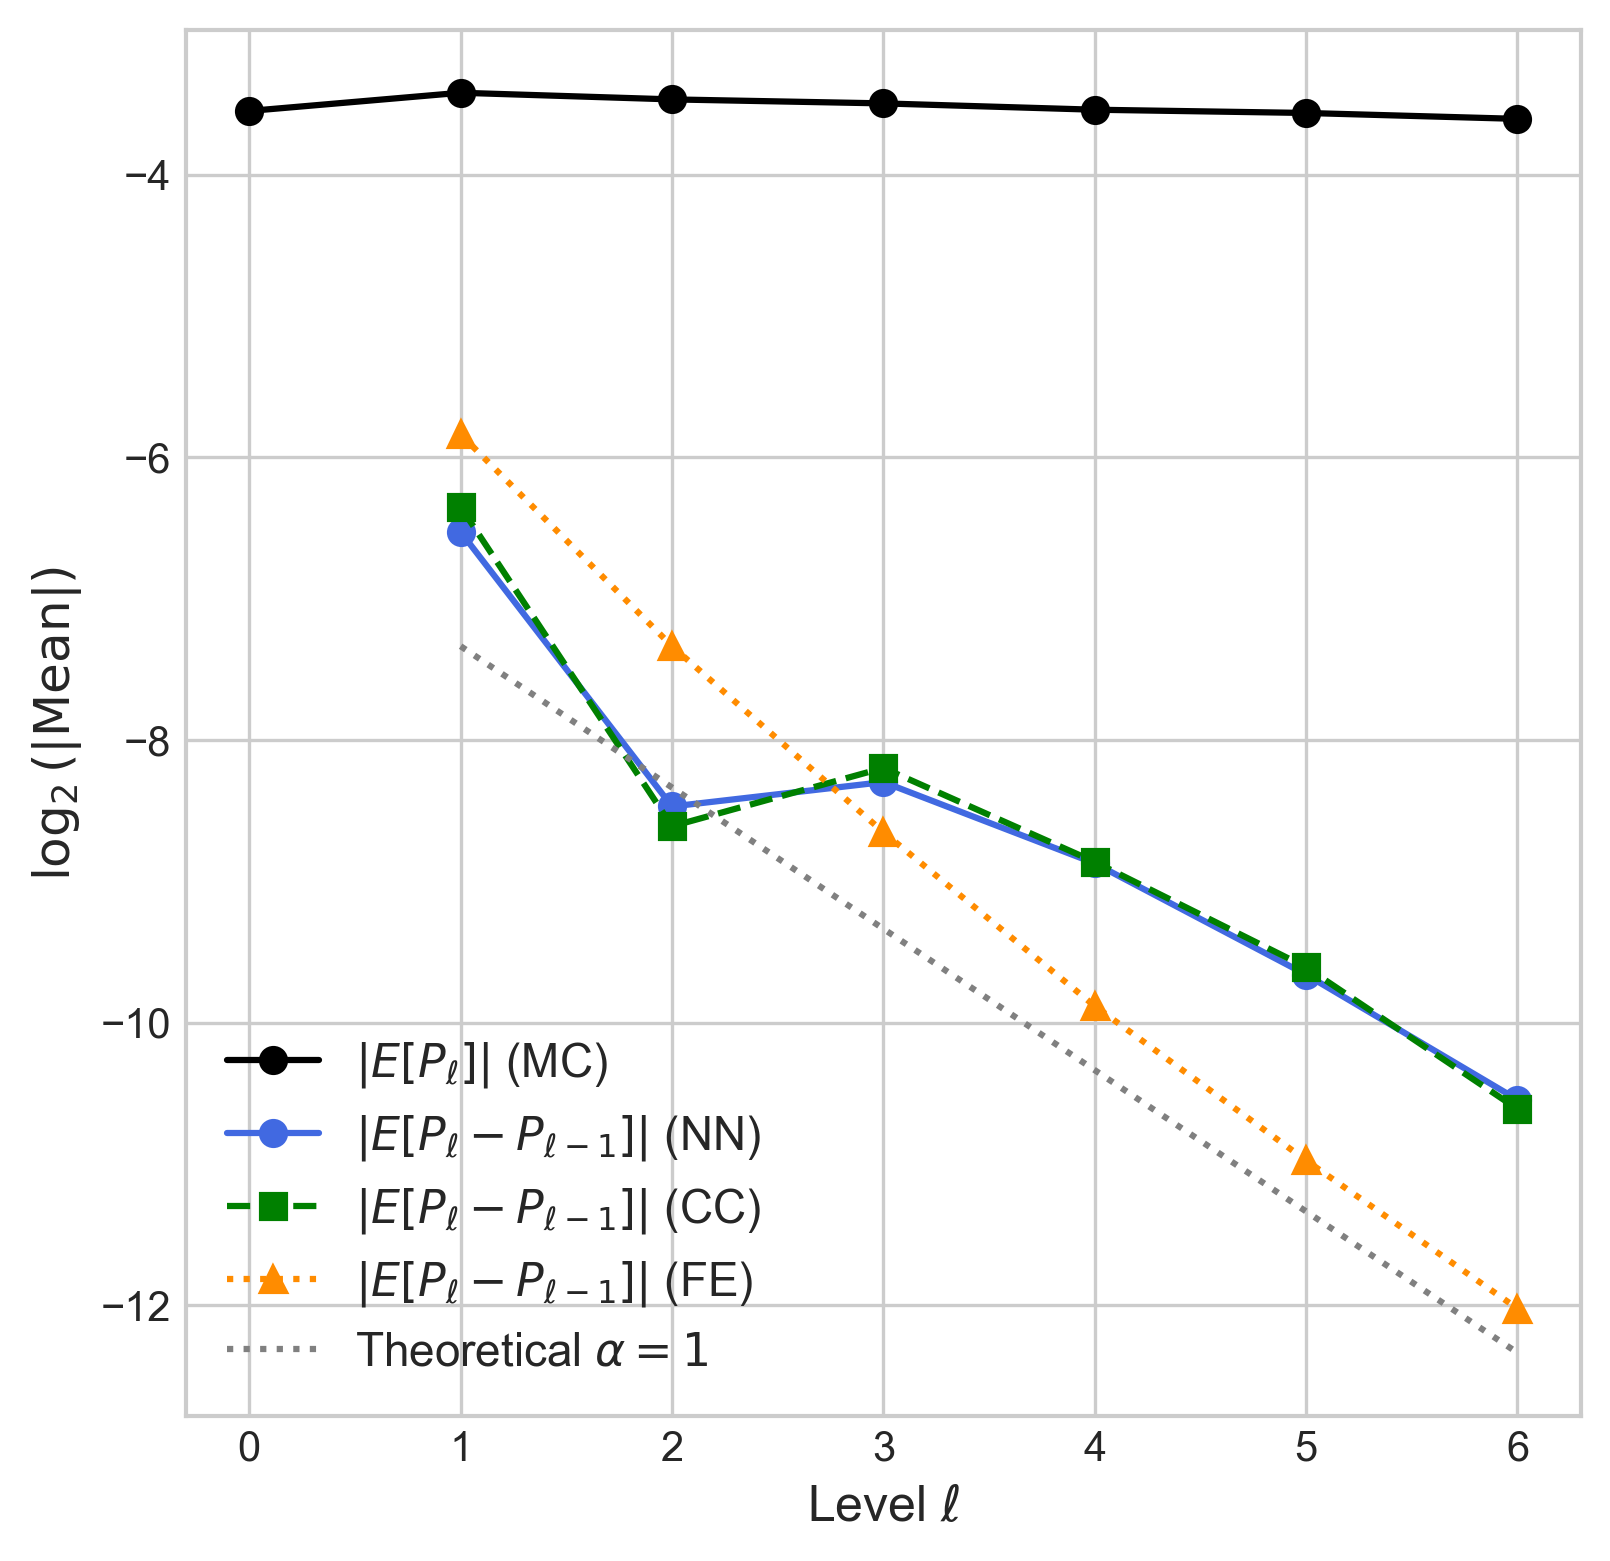
\includegraphics[width=\linewidth]{graphics/she_energy_err_decay.png}
            \caption{Weak error convergence ($\alpha$).}
            \label{fig:mean_decay}
        \end{subfigure}
    \end{subfigure}
    \vspace{1cm}
    \begin{subfigure}{\textwidth}
        \centering
        \begin{subfigure}[b]{\textwidth}
            \centering
            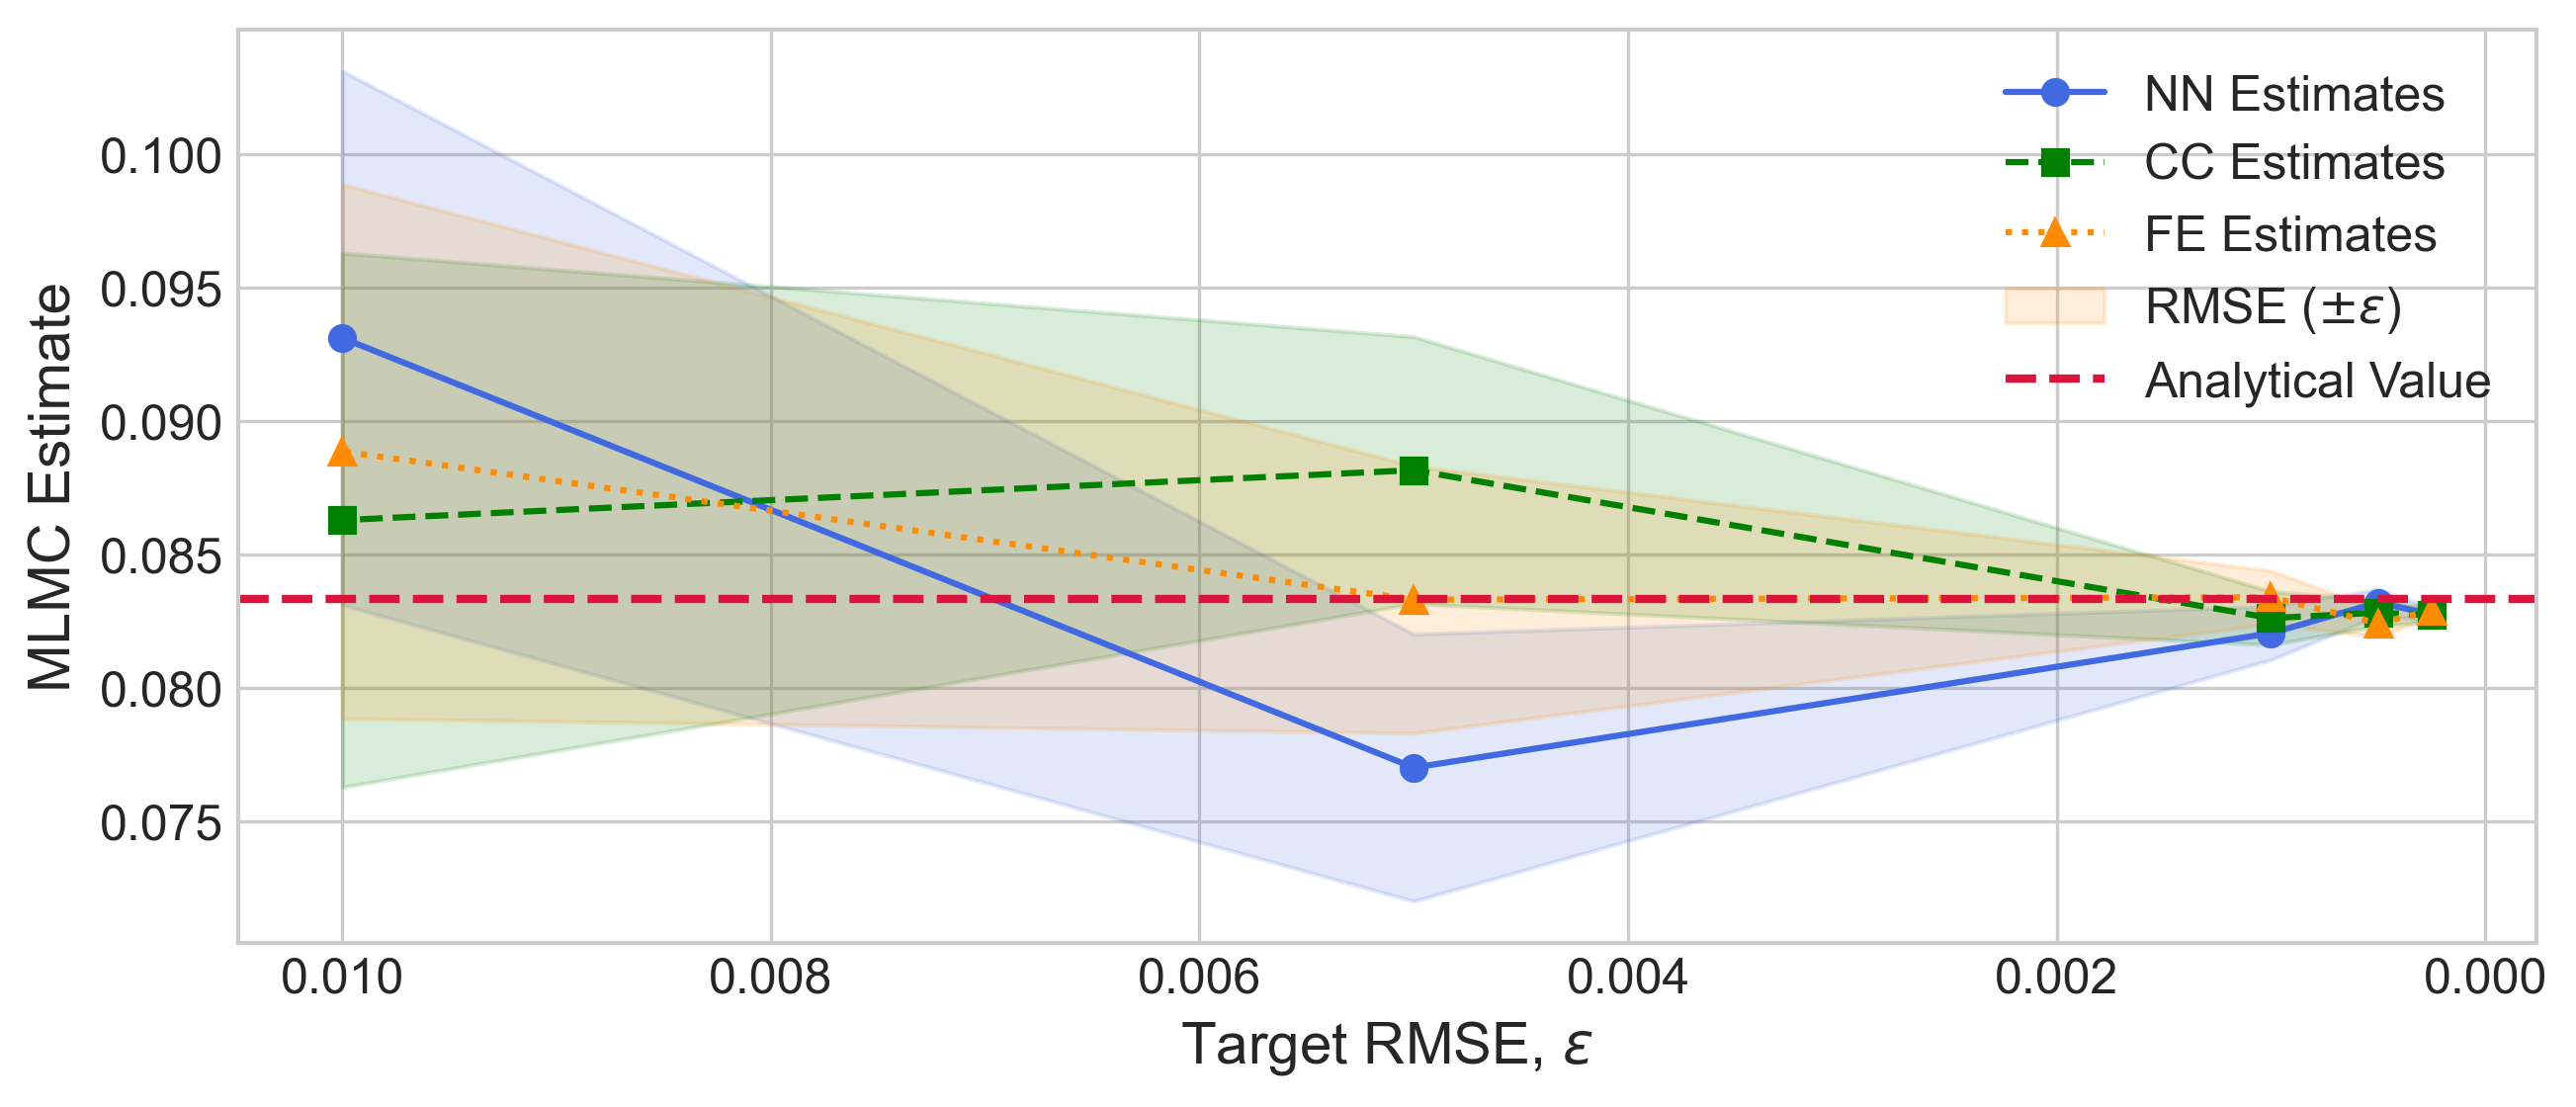
\includegraphics[width=0.7\linewidth]{graphics/she_energy_conv.png}
            \caption{Final MLMC estimate vs. target RMSE ($\varepsilon$).}
            \label{fig:conv_vs_eps}
        \end{subfigure}
        \vspace{0.5cm}
        \begin{subfigure}[b]{\textwidth}
            \centering
            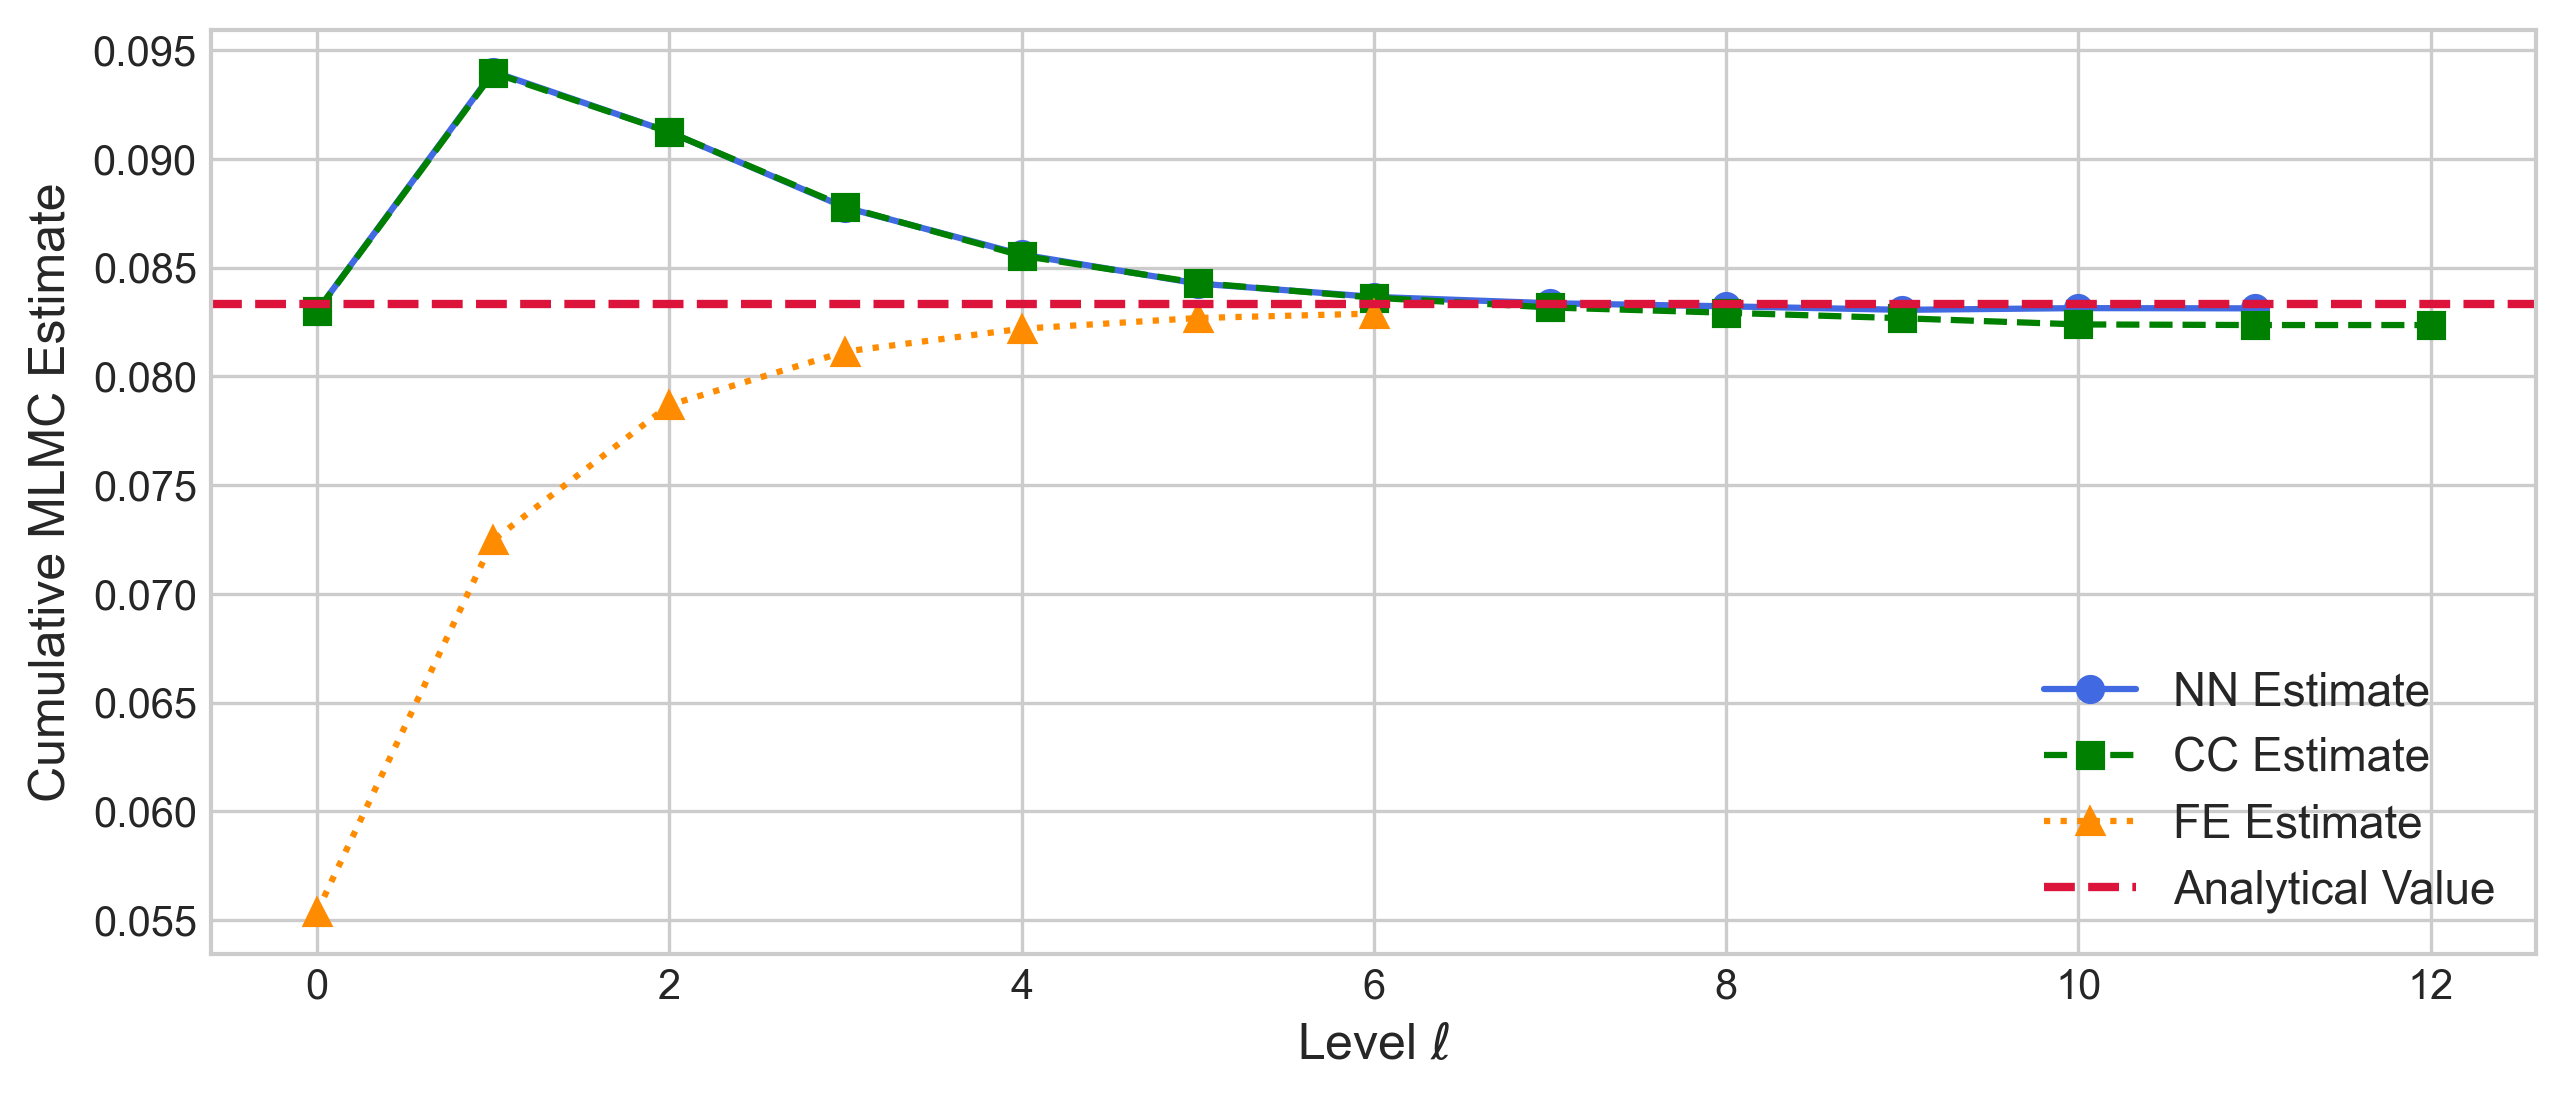
\includegraphics[width=0.7\linewidth]{graphics/she_energy_cumconv.png}
            \caption{Cumulative estimate vs. level ($\ell$) for $\varepsilon=0.001$.}
            \label{fig:cumulative_conv}
        \end{subfigure}
    \end{subfigure}
    \caption{Validation and convergence plots for the MLMC implementation for the SHE, evaluating
    the energy.}
    \label{fig:she_validation_combined}
\end{figure}
